\documentclass{article}
\usepackage{graphicx} % Required for inserting images
\usepackage{hyperref}
\usepackage{cite}          % For better handling of citations
\usepackage{url}           % For handling URLs in references
\usepackage{amsmath}


\begin{document}

\begin{titlepage}
\begin{center} 

        \Huge{Report} \vspace{1cm} 
        
        \large{Pooja Yakkala} \vspace{0.3cm}

        \large{py9363@rit.edu} \vspace{0.3cm} 
        
        
    \end{center} 
\end{titlepage}

\section*{Implementation Description}
To implement the genetic algorithm, I started with initializing the population. I used a different config file that contains the variables written inside the file and the function reads them and maps them to the variables accordingly. I randomly initialized the population with the population size given in the config file. Then I started my implementation of the genetic algorithm. Here in genetic algorithm, we have fitness, crossover and mutation functions. I used the fitness function given in the problem which return value of the chromosome if it is under the weight constraint and it returns 0 if it is over the weight constraint. Here for the first problem, it works fine for the first config file. But for the second config file, the population that is randomly generated is always heavier than the bag weight, so all the fitness rates become 0 and the model no longer improves as the fitness of everything is 0 and as we are only implementing the selection function the parents are copied into the next generation. 

So here, I applied a penalty and repair function which does the following- First, the function checks if the weight is greater than the bag weight. If it is less than the bag weight the value of the chromosome is returned. However, if it is more than the bag weight, then a penalty is applied to the value of the chromosome. This is basically a soft penalty which means that we are not removing the chromosome by giving it a harsh penalty (returning 0) but we taking the chromosome in account by giving it a decrease in the value so that if it becomes better than the solution without any penalty, we can consider it (meaning the population will improve (offspring generations)). However, I have been getting an error for this. The weight of my best solution was becoming more than the weight of the bag. This should not happen as the algorithm should not consider a solution that has weight more than the bag weight as the best solution. I then found out that this error was occurring because my population was changing but it is not getting under the weight constraint. Then I tried repairing my population chromosomes that are over-weight by discarding the gene that has the most weight. Now my genetic algorithm is working as intended getting a solution under then weight constraint.

Then I moved to the roulette and tournament functions. The challenge that I faced here was when all the finesses are 0, the roulette function doesn’t work. As we get a divisible by 0 error. Another one was when I got a negative fitness value. As probabilities can only be non-negative numbers. Here I used random selection to select two parents out of the population whenever the total fitness of the population is 0. For the stop function, I used the method to stop the iterations at the maximum generation and return the Pstop value as intended. Here I observed some graphs with no improvement for several generations. So, the stop criteria that I applied is that when the certain percent of population have the same fitness (meaning they are not improving) the function stops. Lastly, for the population trails, I took 10 to 500 population sizes to see how they are varying in their knapsack value. It can be seen how different population sizes have an effect on the knapsack problem. For the non-genetic algorithm, I chose to do Dynamic Programming which gives fast and optimal solutions and compared it with my GA algorithm.

\section*{Selection Alone}
	First of all, I ran my selection alone algorithm on config 1. Each of my graphs contain a comparison between roulette data and tournament data. From the first two graphs, we can see that there is no difference between generation 0 till generation 25. The best solution is found at gen 0 and the parents are copied to all the generations in this function. Hence, we have the same fitness for the fittest and same number of active genes through out the generations. Then when running the config 2, I got all the fitnesses as 0 because the weight of the gen 0 is over the limit of the bag. And the same chromosome is copied to all the generations so the fitness is also same. But the active genes are different, that it, here as the fitness is zero, we select two randomly, then they get added to a new population where the process repeats so every time the parents changes their active genes are different but since all of them are over-weight there is not change in the fitness. Also, we can see that in the selection only function, the Pstop is same as the best solution (Generation 0). By seeing these results, I can tell that without the crossover or mutation and simply with selection the model can never improve. It just passes on the same parents to the child generations.
 \begin{figure}[h]
    \centering
    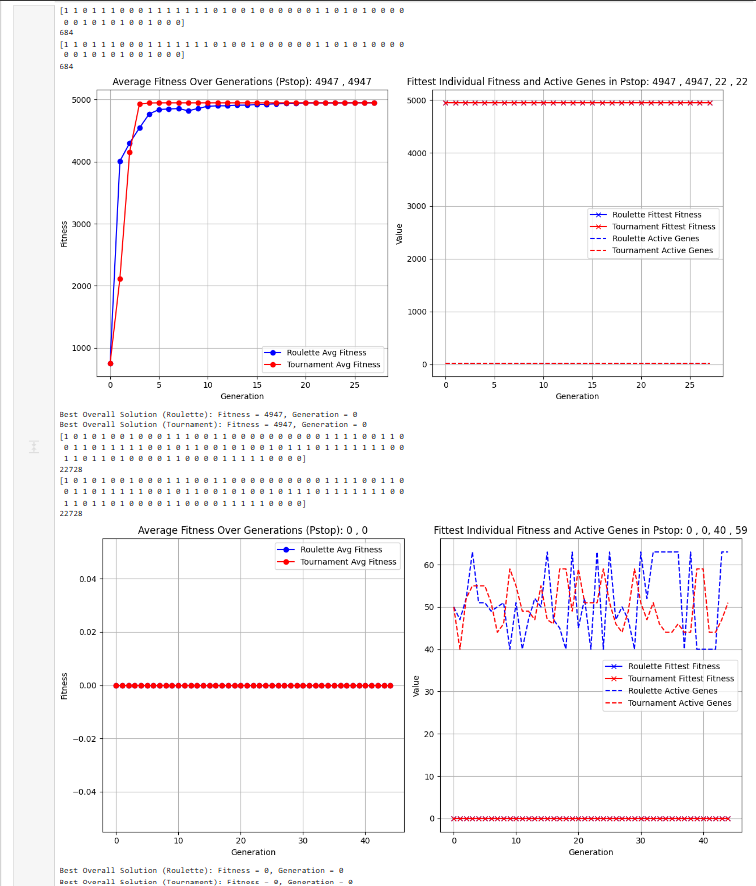
\includegraphics[width=0.5\linewidth]{q1.png}
    \caption{Selection Alone}
    \label{fig:enter-label}
\end{figure}

\section*{Custom Fitness Function}
	Applying the custom fitness function, we can see that there is an improvement in the config 2. Initially the fitness was zero but now the fitness has increased. But the fitness remains constant throughout again because this is selection only and the parents are being copied to the next generation. Also, we know that if there is a large gap between the Pstop and the average fitness of the entire population, the model is not performing well. And the same thing happened here between the 0 to 10th generations in config 1 and after which the performance is constant.
 \begin{figure}[h]
    \centering
    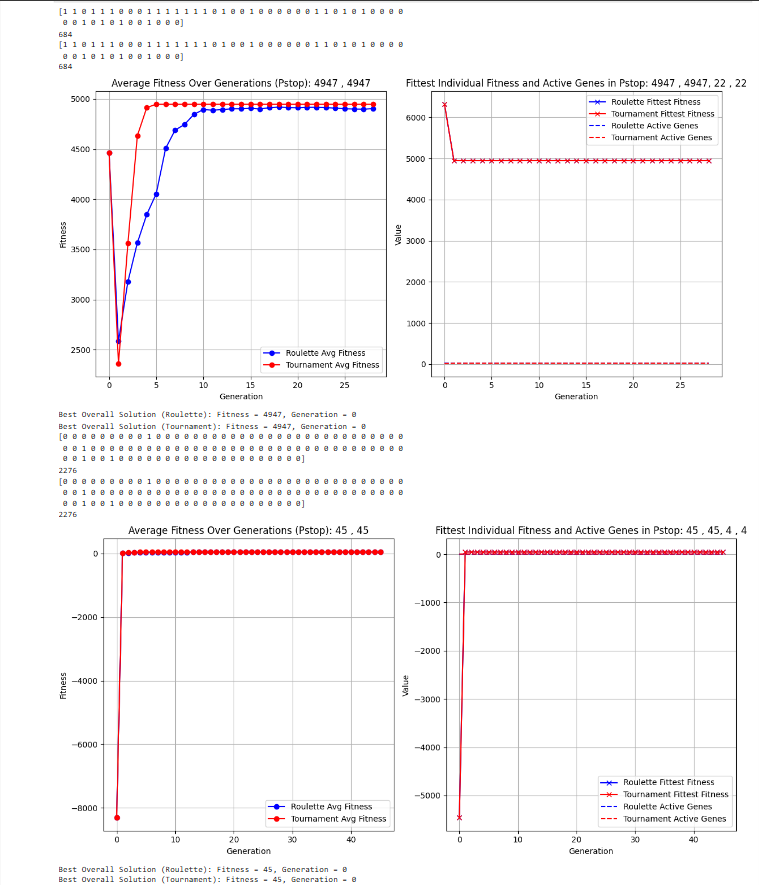
\includegraphics[width=0.5\linewidth]{q2.png}
    \caption{EC}
    \label{fig:enter-label}
\end{figure}

\section*{Integrate Cross-over and Mutation}
	Upon adding the crossover and mutation (without the fitness function), there is a significant change in the graphs which shows the model is improving. This can be seen in the results as the best fitness increases to 5598 in roulette and 7142 in tournament (for mutation rate 0.05 and config 1). Comparing this to the previous selection only function (without custom fitness), we can see that both roulette and tournament functions give 4947. I have performed the function on different mutation rates and note that the mutation rate of 0.2 bring the most optimal solution for config 1 with roulette. While mutation rate of 0.1 is best for config 1 with tournament. Similarly, mutation rate of 0.05 gives the optimal solution for both roulette and tournament in config 2. My observations are that, by implementing crossover and mutation we are ensuring that the offsprings are improving and not copying the parents to the new generation. This gives a diverse population and hence, we have a smaller difference the Pstop and the average fitness across all generations. Another point is that, tournament method gave high fitness values with lower mutation rate(0.05), which shows that it is more effective at preserving best individuals but still introduces diversity to the population. Then I applied my custom fitness function to the crossover and mutation functions. The results are as follows, the optimal solution is found at mutation rate 0.05 for the roulette function and tournament functions for config 1. While the optimal solution for config 2 is 0.10 for roulette and 0.05 for tournament. 
\begin{figure}
    \centering
    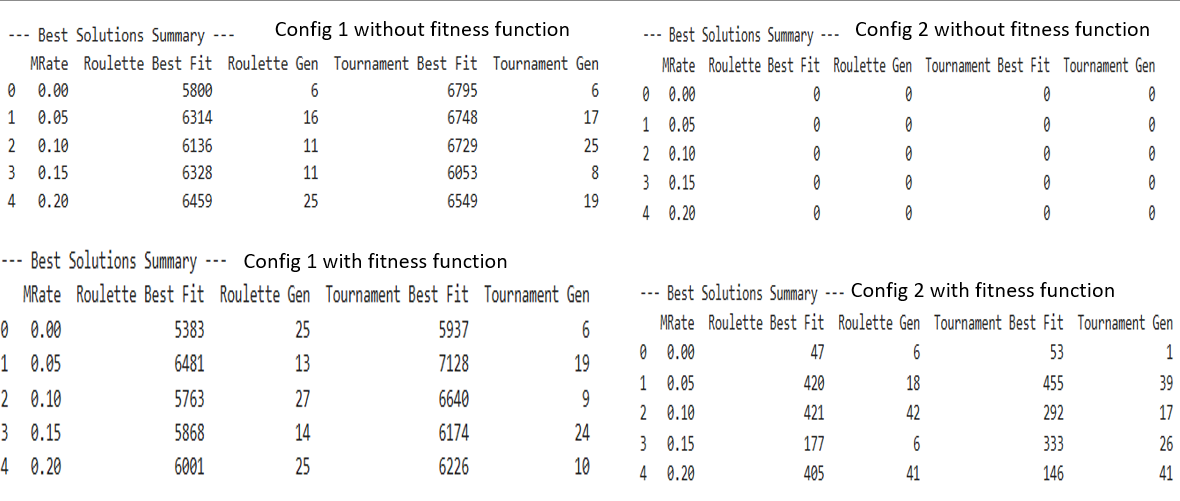
\includegraphics[width=1\linewidth]{q3.png}
    \caption{Cross-Over and Mutation}
    \label{fig:enter-label}
\end{figure}
\section*{Custom Stop Criteria}
	For the stop criteria, I implemented a criterion where the algorithm stops when the population no longer improves. Applying this on normal fitness function, I observed that it gives me the most optimal solution when compared to the normal stop criteria and it shows the point where the model stops improving. For config 2, as the fitness is always 0 here, the model converges at generation 0. Now, when I implement the custom stop criteria with my custom fitness function, we can see that the model is improving and it doesn’t converge much as the population is diverse and the model can search for a more optimal solution here and avoid the local optima. The results with respect to mutation rates is given.
\begin{figure}
    \centering
    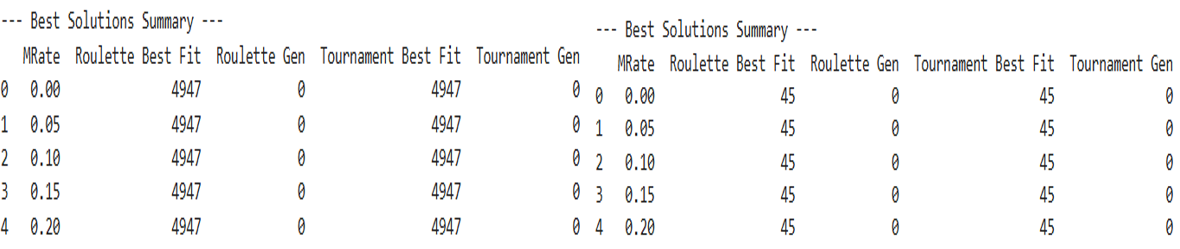
\includegraphics[width=1\linewidth]{q3 ec.png}
    \caption{EC}
    \label{fig:enter-label}
\end{figure}

\section*{Comparing GA with a Non-population-based Search Algorithm}
\section*{Exploring Population Sizes}
The following are the results of performing the algorithm with different population sizes. As we can see, different population sizes have different impacts on the solution. The mean knapsack value increases but then gets stable after a certain point. Also, that in both the tables we can see that the sizes 50 and 75 give the optimal solutions and increasing the population size doesn’t mean that it increases the fitness value. 
\begin{figure}[h]
    \centering
    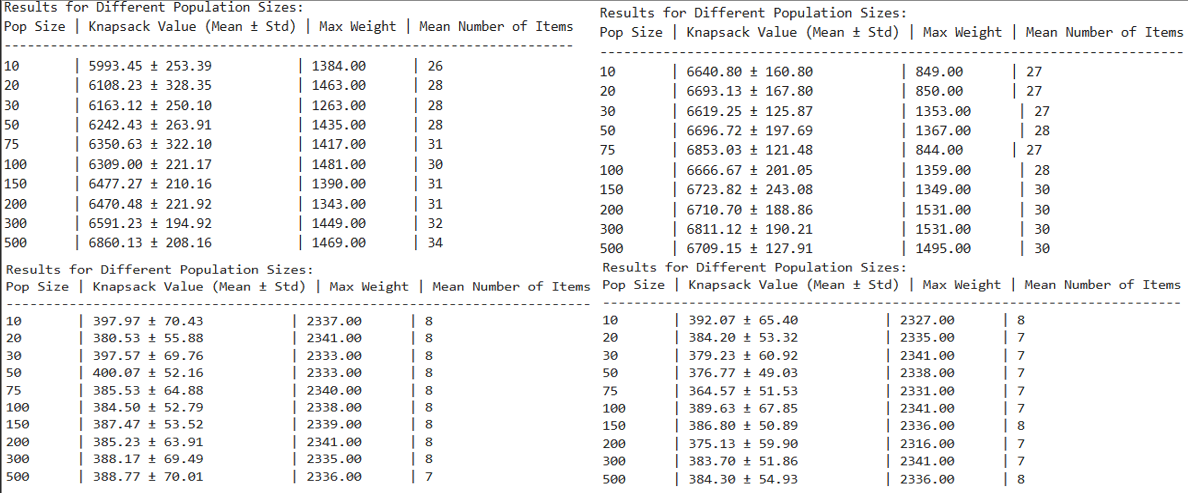
\includegraphics[width=1\linewidth]{q4.png}
    \caption{Population Sizes}
    \label{fig:enter-label}
\end{figure}

\section*{Comparing GA with a Non-population-based Search Algorithm}
	I have chosen Dynamic Programming for the Non-Genetic Algorithm. Upon comparison, we can see that Dynamic programming is way faster than Genetic Algorithms. It is easier to implement as it just computes the values based on the constraints of the problem but this also makes it quite inflexible. It did really well on the smaller config files provided but DP are generally known for their memory consumption so it is not the best. Here Genetic Algorithm gave a better solution than Dynamic programming as we can see. They are flexible and also good for large data. However, they are slow and there is no guarantee that the solution we found is the optimal as it depends on various factors like mutation, crossover and population size etc.
\begin{figure}
    \centering
    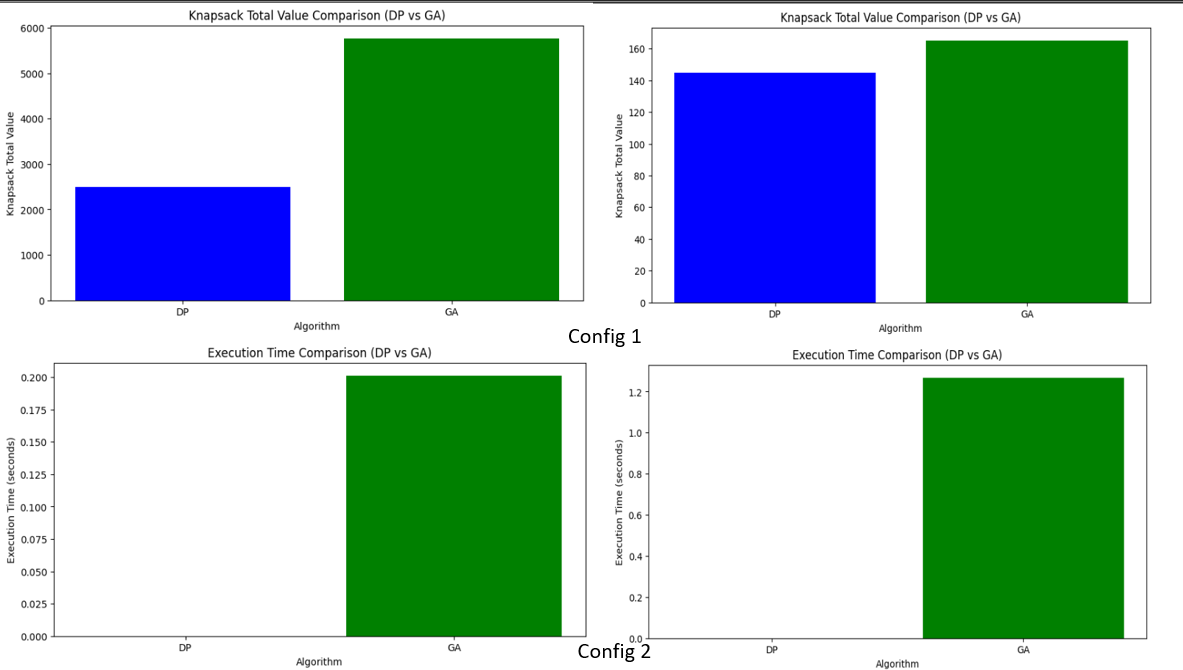
\includegraphics[width=1\linewidth]{q5e.png}
    \caption{Non-population Based Algorithm}
    \label{fig:enter-label}
\end{figure}

\section*{Exploring Another Technique}
\section*{Exploring Another Nature-inspired Search/Optimization Technique}
In this paper the authors introduce an optimization technique that is inspired by honey bees' foraging behavior to tackle complex optimization tasks efficiently. This algorithm relies on the population which imitates the way bees naturally behave by having scout bees venture out into a search area to find the best solutions, that is, by discovering flower patches abundant in nectar. Once they find a spot, the scout bee heads back to the hive and does a "wiggle dance" to show other bees the direction, distance, and quality of that location so they can focus their search, on these productive areas. This method successfully combines investigation of top-notch locations nearby with exploration, by keeping a few scouts, for random searches to enhance the chances of finding the best solution. 

The Bees Algorithm uses swarm intelligence principles, like other optimization methods such as Particle Swarm Optimization, Ant Colony Optimization, and Genetic Algorithms. This method sets itself apart by blending neighborhood search with a more extensive exploration approach to escape from local optima effectively. During each cycle of the algorithm process, the scout bees assess the quality of discovered locations, and then prime areas are chosen for neighborhood search. All the other additional bees are tasked with searching around these promising spots. This process repeats until it reaches a specific stopping point. The stop point can be like reaching several iterations or achieving a level of success in fitness tests. This approach offers flexible methods by concentrating more on key areas and also exploring new territories thereby giving effective solutions for resolving complex situations with multi-modal problems. 

The authors compared the effectiveness of this algorithm against complex functions like Shekel’s Foxholes and the Schwefel function and stated that this technique is more effective when compared with the others. During these tests, the Bees Algorithm consistently surpasses optimization techniques by converging quickly and achieving a higher rate of success. Its distinct structure allows it to adaptively distribute resources according to the effectiveness of each solution while keeping diversity in the search area by keeping scout bees to investigate regions. Fine-tuning aspects such as the number of scout bees, the size of their neighborhoods, and the elite site selection in the algorithm is essential for performance in swarm-based optimization tasks. Its nature inspired that enhances both speed and precision of solutions offered by the Bees Algorithm—a versatile tool adept at tackling intricate problems with multiple variables by mimicking bee search strategies effectively.
\bibliographystyle{plain}
\bibliography{paper} 
\href{https://www.sciencedirect.com/science/article/abs/pii/B978008045157250081X}{
D.T. Pham, A. Ghanbarzadeh, E. Koç, S. Otri, S. Rahim, M. Zaidi, The Bees Algorithm — A Novel Tool for Complex Optimisation Problems, Intelligent Production Machines and Systems, 2nd I*PROMS Virtual International Conference 3–14 July 2006. Pages 454-459}
\end{document}
